% This is LLNCS.DEM the demonstration file of
% the LaTeX macro package from Springer-Verlag
% for Lecture Notes in Computer Science,
% version 2.4 for LaTeX2e as of 16. April 2010
%
\documentclass{llncs}
%
\usepackage{multirow}
\usepackage{hhline}
\usepackage{caption}
\usepackage{makecell}
\usepackage{ragged2e}
\usepackage{parskip}
\usepackage{wrapfig}
\usepackage{array}
\usepackage{float}
\usepackage[english]{babel}
\usepackage{lipsum}
\usepackage{caption}
\usepackage{subcaption}
\usepackage{graphicx}
\graphicspath{{images/}} 
\usepackage[linesnumbered,ruled]{algorithm2e}
\usepackage{courier}
\usepackage{hyperref}
\hypersetup{colorlinks=true,allcolors=blue}
\usepackage{listings}
\usepackage{float}
\lstset{
    basicstyle=\ttfamily,
    frame=none, 
    breaklines=true,
    numbers=left,
    xleftmargin=2.5em,
    framexleftmargin=0em,
    emphstyle=\textbf,
    float=t
}
\lstdefinestyle{ocl}{
    emph={
        context, inv
    }
}
\lstdefinestyle{cbp}{
    basicstyle=\ttfamily\scriptsize,
    emph={
        session, create, type,
        set, to, add, hire
    }
}
\lstdefinestyle{xmi}{
    basicstyle=\ttfamily\scriptsize,
    emph={
        Node, children
    }
}
\lstdefinestyle{xml}{
    basicstyle=\ttfamily\scriptsize,
    emph={
        register, create, add, to, resource,
        from, eattribute, remove, ereference,
        set, unset, session, Roy, Jen,
        Moss, Richmond
    }
}
\lstdefinestyle{java}{
    basicstyle=\ttfamily\scriptsize,
    emph={
        case, $unset$,
        instanceof, else, if, void,
        new, UnsetEAttributeEvent,
        UnsetEReferenceEvent,
        @override, public, class, extends
    }
}
\lstdefinestyle{eol}{
    basicstyle=\ttfamily\scriptsize,
    emph={
        var, new, for, in, create, set, with, type,
        unset, to, add, remove, delete, register, move,
        from, position, from, move-within, session, \.
    }
}

% $ChangeHybridEventAdapter$

\hyphenation{op-tical net-works semi-conduc-tor Hybrid-Change-Event-Adapter Hybrid-XMI-Change-Event-Adapater
    Hybrid-Neo-EMF-Change-Event-Adapater change-Events Change-Event-Adapter EContent-Adapter notify-Changed Hybrid-Resource Resource-Impl state-Based-Resource cbp-Output-Stream Output-Stream Hybrid-Change-Event-Adapater Output-Stream Hybrid-XMI-Resource-Impl Hybrid-Neo-EMF-Resource-Impl Persistence-Resource change-Events
}


\begin{document}
\renewcommand{\thelstlisting}{\arabic{lstlisting}}
\renewcommand{\labelitemi}{$\bullet$}
\newcommand{\dk}[1]{\textbf{[DK: #1]}}

\title{Harnessing Change-based Persistence for\\Faster Model Comparison}
%
\titlerunning{Towards Change-based Model Comparison}  % abbreviated title (for running head)
%     also used for the TOC unless
%     \toctitle is used
%
\author{
Alfa Yohannis \and Horacio Hoyos Rodriguez$^{*}$ \and Fiona Polack$^{**}$ \and \\ Dimitris Kolovos
}

%\author{
%Alfa Yohannis$^{1,3}$ \and Horacio Hoyos Rodriguez$^{*1}$ \and Fiona Polack$^{**2}$ \and \\ Dimitris Kolovos$^{1}$
%}
%
\authorrunning{
Alfa Yohannis et al.
} % abbreviated author list (for running head)
%
%%%% list of authors for the TOC (use if author list has to be modified)
%\tocauthor{Alfa Yohannis,Horacio Hoyos Rodriguez, Fiona Polack, Dimitris Kolovos}
%\institute{anonym}

\institute{Department of Computer Science, University of York, United Kingdom\\
    $^{**}$School of Computing and Maths, Keele University, United Kingdom\\
\email{\{ary506, dimitris.kolovos\}@york.ac.uk
\\$^{*}$horacio\_hoyos\_rodriguez@ieee.org
\\$^{**}$f.a.c.polack@keele.ac.uk}}

%\institute{$^{1}$Department of Computer Science, University of York, United Kingdom\\
%    $^{2}$School of Computing and Maths, Keele University, United Kingdom\\
%    $^{3}$Department of Computer Science, Institut Teknologi dan Bisnis Kalbis, Indonesia\\
%    \email{\{ary506, dimitris.kolovos\}@york.ac.uk
%        \\$^{*}$horacio\_hoyos\_rodriguez@ieee.org
%        \\$^{**}$f.a.c.polack@keele.ac.uk}}

\maketitle      % typeset the title of the contribution

%The first states the problem. The second states why the problem is a problem. The third is my startling sentence. The fourth states the implication of my startling sentence.
\begin{abstract}
Comparison of two large state-based models can be time-consuming since every element of a model has to be visited, matched, and diffed with its respective element on the other model. This downside causes a bottleneck in collaborative modelling especially when identifying differences between two versions of a model is desirable. This paper harnesses change-based persistence to localise the comparison of models so that only elements affected by recent changes that are compared. This approach leads to a faster model differencing as opposed to the traditional state-based model comparison. 
\end{abstract}

\vspace{-20pt}
\section{Introduction}
\label{sec:introduction}
In the context of collaborative modelling, large models are often developed in parallel with different modellers working on certain parts. This condition leads to the existence of different versions of the models. Further, in the integration process, these different versions of models need to be compared to identify their differences and to check if there are conflicts when merging them. Comparing these large models in state-based format can be lengthy since every element of a model has to be visited, matched, and diffed with its respective element on the opposite model. 
This lengthy comparison can slow down the construction of models in a collaborative modelling setting. 

In this paper, we present our approach in harnessing change-based persistence (CBP) to optimise model comparison. The nature of CBP that records recent changes with detailed information facilitates the identification of elements that have been changed since the last version. The availability of this information eliminates the necessity to visit, match, and diff \textbf{every} element of models being compared. Thus, we can localise model comparison only to recently affected elements which in turns can reduce the time used for model comparison. 

This paper is structured as follows. Section \ref{sec:change-based_persistence} introduces the concept of change-based persistence. Sections \ref{sec:change-based_model_comparison} and \ref{sec:implementation} present our change-based approach to optimise model comparison and its implementation. Section \ref{sec:evaluation} presents our experimental results and evaluation. Section \ref{sec:related_work} provides an overview of related work, and Section \ref{sec:conclusion_and_future_work} concludes with a discussion on directions for future work.


\section{Change-based Persistence}
\label{sec:change-based_persistence}

\begin{minipage}[t]{0.59\linewidth} 
\centering
\begin{lstlisting}[style=eol,caption={The simplified XMI of the model in Fig. \ref{fig:origin}.},label=lst:originxmi]
<uml:Class id="c" name="Class 1">
 <operation id="oa" name="Operation A"/>
 <operation id="ob" name="Operation B"/>
 <operation id="oc" name="Operation C"/>
 <operation id="od" name="Operation D"/>
 <operation id="oe" name="Operation E"/>
</uml:Class>
\end{lstlisting}
\vspace{-25pt}
\begin{figure}[H]
\centering    
\hfill
\begin{subfigure}[t]{0.2\linewidth}
    \centering
    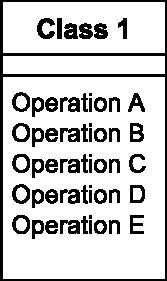
\includegraphics[width=\linewidth]{images/OriginalClassDiagram}
    \caption{origin}
    \label{fig:origin}
\end{subfigure}
\hfill
\begin{subfigure}[t]{0.2\linewidth}
    \centering
    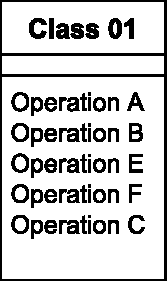
\includegraphics[width=\linewidth]{images/LeftClassDiagram}
    \caption{left}
    \label{fig:left}
\end{subfigure}
\hfill
\begin{subfigure}[t]{0.2\linewidth}
    \centering
    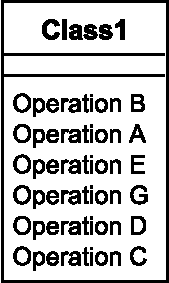
\includegraphics[width=\linewidth]{images/RightClassDiagram}
    \caption{right}
    \label{fig:right}
\end{subfigure}
\hfill
\label{fig:versions}
\caption{Different versions of a model.}
\end{figure}
\end{minipage}
\hfill
\begin{minipage}[t]{0.39\linewidth}
\begin{lstlisting}[style=eol,caption={The pseudo-formatted CBP of the model in Fig. \ref{fig:origin}.},label=lst:origincbp]
session "origin"
create c type Class
set c.name to "Class 1" 
create oa type Operation
set oa.name to "Operation A" 
create ob type Operation
set ob.name to "Operation B" 
create oc type Operation
set oc.name to "Operation C" 
create od type Operation
set od.name to "Operation D" 
create oe type Operation
set oe.name to "Operation E" 
add oa to c.operations
add ob to c.operations
add oc to c.operations
add od to c.operations
add oe to c.operations
\end{lstlisting}
\end{minipage}

Change-based persistence is an alternative approach to the common state-based persistence (SBP) of models. Instead of persisting the last state of a model, CBP persists the overall history of changes of a model. For example, in SBP approach, when we save the UML class diagram in Fig. \ref{fig:origin} in standard XMI format, we only obtain the last state of the model the Listing \ref{lst:originxmi} shows. In contrast, when we develop the model in CBP approach, a system captures all the changes made to the model and persists them into a CBP file as showed in List. \ref{lst:origincbp}. The file consists of events generated by changes. Each event contains information about the type of the operation applied as well the as values, elements, or features involved. Replaying the events in List. \ref{lst:origincbp} produces the same model as in Fig. \ref{fig:origin}.

\section{Model Comparison}
\label{sec:model_comparison}
In the context of collaborative modelling, a model is commonly developed in parallel -- thus produces different versions. Let's say that the model in Fig. \ref{fig:origin} is modified by two different modellers in parallel. The first modeller produces the model in Fig. \ref{fig:left}, and the second one yields the model in Fig. \ref{fig:right} producing XMI files as depicted in Fig. \ref{fig:left} and Fig. \ref{fig:right} respectively.

\begin{minipage}[t]{0.49\linewidth} 
\begin{lstlisting}[style=eol,caption={The simplified XMI of the model in Fig. \ref{fig:left}.},label=lst:leftxmi]
<uml:Class id="c" name="Class 01">
  <operation id="oa" 
    name="Operation A"/>
  <operation id="ob" 
    name="Operation B"/>
  <operation id="oe" 
    name="Operation E"/>
  <operation id="of" 
    name="Operation F"/>
  <operation id="oc" 
    name="Operation C"/>
</uml:Class>
\end{lstlisting}
\end{minipage}
\hfill
\begin{minipage}[t]{0.49\linewidth}
\begin{lstlisting}[style=eol,caption={The simplified XMI of the model in Fig. \ref{fig:right}.},label=lst:rightxmi]
<uml:Class id="c" name="Class1">
  <operation id="ob" 
    name="Operation B"/>
  <operation id="oa" 
    name="Operation A"/>
  <operation id="oe" 
    name="Operation E"/>
  <operation id="og" 
    name="Operation G"/>
  <operation id="od" 
    name="Operation D"/>
  <operation id="oc" 
    name="Operation C"/>
</uml:Class>
\end{lstlisting}
\end{minipage}

At some point, these two models needs to be compared (e.g. to identify their differences for analytics or conflicts when merging). The common approach to compare both models is to create matches between the elements of both models and diff them. Commonly, the matching process matches elements by using their identifiers or through a distance mechanism if they have none \cite{}. The diffing process 

\section{Implementation}
\label{sec:implementation}

\begin{figure}
    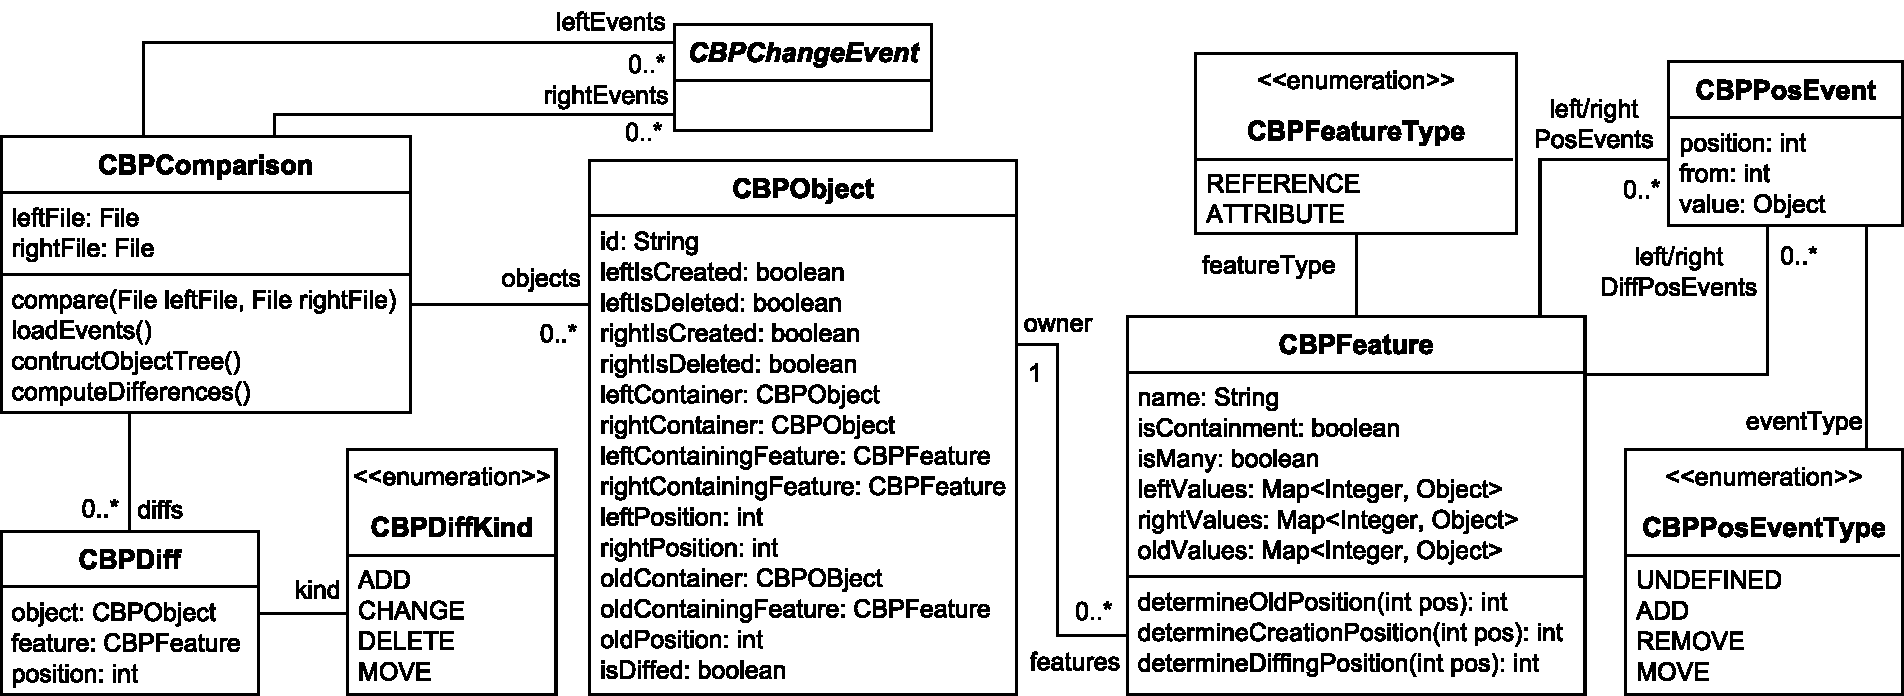
\includegraphics[width=\linewidth]{images/TreeClassDiagram}
    \caption{A class diagram showing the core components of the change-based approach to optimise model comparison.}
    \label{fig:approach_class_diagram}
\end{figure}

\section{Change-based Model Comparison}
\label{sec:change-based_model_comparison}

\begin{minipage}[t]{0.49\linewidth}    
\begin{lstlisting}[firstnumber=24,style=eol,caption={The left version.},label=lst:leftcbp]
session "LEFT"
set c.name from "Class 1" to "Class 01"
move oc in c.operations from 2 to 4
unset od.class from oc to null
remove od from c.operations
delete od
create of type Operation
set of.name to "Operation F"
add of to c.operations
\end{lstlisting}
\end{minipage}
\hfill
\begin{minipage}[t]{0.49\linewidth}
\begin{lstlisting}[firstnumber=24,style=eol,caption={The right version.},label=lst:rightcbp]
session "RIGHT"
set ob.name from "Operation B" to "Operation BB"
move oc in c.operations from 2 to 4
move oe in c.operations from 3 to 2
create og type Operation
set og.name to "Operation G" 
add og to c.operations pos 3
move ob in c.operations from 1 to 0
set oa.name from "Operation BB" to "Operation B"
set c.name from "Class 1" to "Class1"
\end{lstlisting}
\end{minipage}

\begin{figure}
    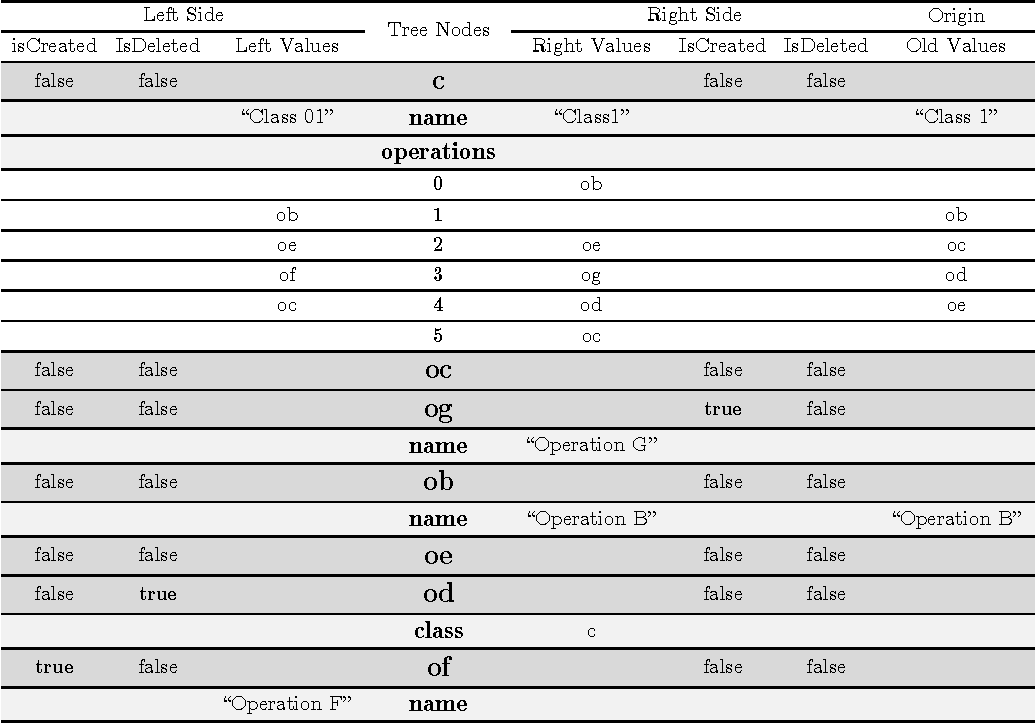
\includegraphics[width=\linewidth]{images/TreeTableCropped}
    \caption{A table showing the state of the object tree of both CBPs in List. \ref{lst:leftcbp} and List. \ref{lst:rightcbp}.}
    \label{fig:class_diagram}
\end{figure}



\section{Evaluation}
\label{sec:evaluation}


\begin{figure}
\hfill
\centering    
\begin{subfigure}[t]{\linewidth}
    \centering
    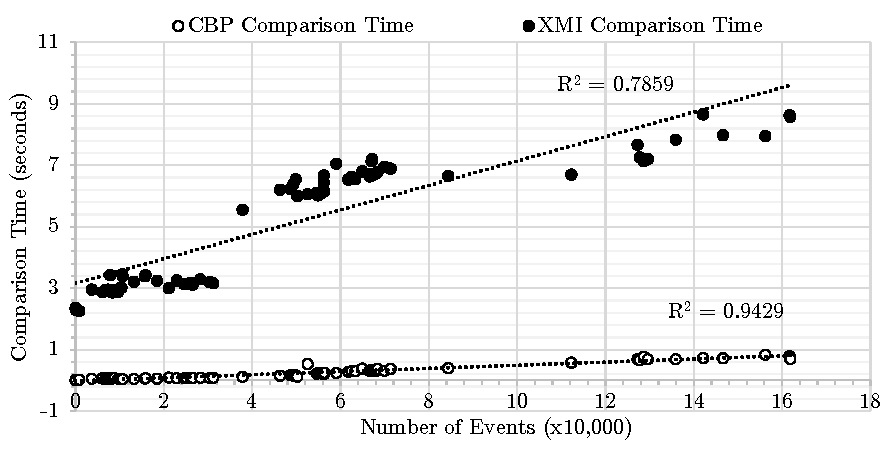
\includegraphics[width=\linewidth]{images/Time-Events}
    \caption{comparison time vs. number of events}
    \label{fig:time_events}
\end{subfigure}
\hfill
\centering    
\begin{subfigure}[t]{\linewidth}
    \centering
    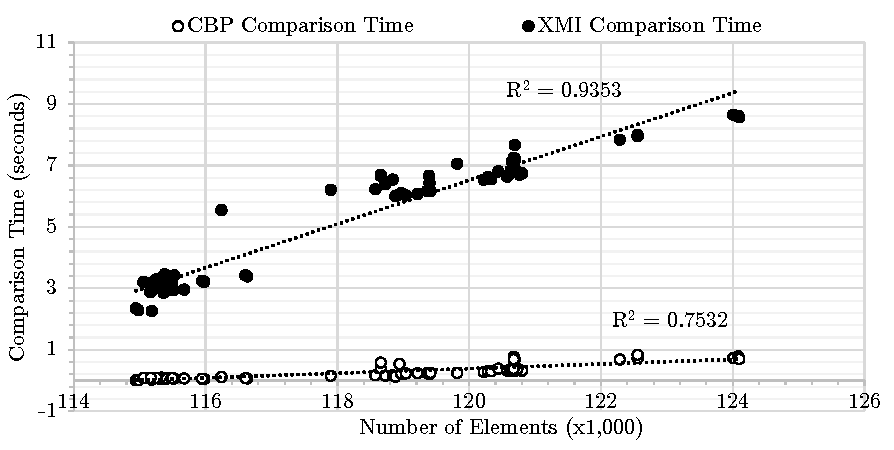
\includegraphics[width=\linewidth]{images/Time-Elements}
    \caption{comparison time vs. number of elements}
    \label{fig:time_elements}
\end{subfigure}
\\
\hfill
\centering    
\begin{subfigure}[t]{\linewidth}
    \centering
    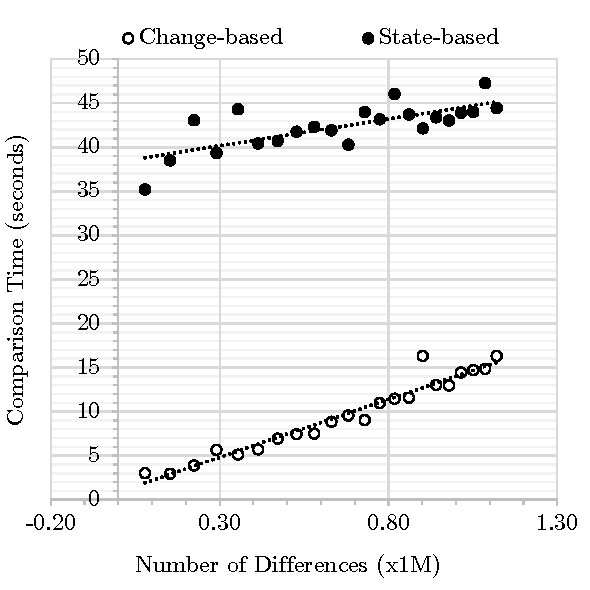
\includegraphics[width=\linewidth]{images/Time-Diffs}
    \caption{comparison time vs. number of diffs}
    \label{fig:time_diffs}
\end{subfigure}
\hfill
\label{fig:perfomance_evaluation}
\caption{Comparison between CBP and XMI on model comparison time.}
\end{figure}

\subsection{Limitation and Threat to Validity}
\label{sec:limitation_and_Threat_to_validity}

\section{Related Work}
\label{sec:related_work}

Comparison at the structural level. EMF Compare, SiDiff, ECL. 

EMFStore
Comparison at the change/operational level. 

Our approach use the changes to compare at the structural level.


\section{Conclusions and Future Work}
\label{sec:conclusion_and_future_work}


\cite{DBLP:conf/caise/IgnatN05}

\vspace{-10pt}
\subsubsection*{Acknowledgements.} This work was partly supported by through a scholarship managed by \emph{Lembaga Pengelola Dana Pendidikan Indonesia} (Indonesia Endowment Fund for Education).
%\clearpage

\bibliography{references} 
\bibliographystyle{splncs}

\end{document} 
